\documentclass[10pt,journal,compsoc]{IEEEtran}

\usepackage{amsmath,amssymb,amsfonts}
\usepackage{algorithmic}
\usepackage{graphicx}
\usepackage{textcomp}
\usepackage{xcolor}
\usepackage{booktabs}
\usepackage{hyperref}
\usepackage{microtype}
\usepackage{cite}
\usepackage{tikz}
\usetikzlibrary{shapes.geometric, arrows.meta, positioning}

\hypersetup{
    colorlinks=true,
    linkcolor=blue,
    citecolor=blue,
    urlcolor=teal
}

\begin{document}

\title{Fast-DINO-AD: High-Throughput Edge Industrial Anomaly Detection via Multi-Scale Vision Transformers and Quantized Vector Memory Banks}

\author{Meryam~Benalia%
\thanks{M. Benalia is the author and lead researcher of Fast-DINO-AD. E-mail: mi.benalia@gmail.com. Project repository: \url{https://github.com/meryambn/Fast-Dino-ad}}%
}

\markboth{IEEE Transactions on Industrial Informatics (Preprint), March 2026}%
{Benalia: Fast-DINO-AD: High-Throughput Edge Industrial Anomaly Detection}

\IEEEtitleabstractindextext{%
\begin{abstract}
Automated optical inspection (AOI) on industrial assembly lines demands sub-hundred-millisecond inference latency, minimal memory footprints for embedded compute, and sub-millimeter anomaly localization without access to defective training data. Traditional patch-based nearest-neighbor architectures such as PatchCore achieve competitive area-under-the-receiver-operating-characteristic (AUROC) scores on benchmarks like MVTec AD, yet suffer from severe deployment bottlenecks: linear retrieval latency $O(N)$ against dense uncompressed float32 patch embeddings, hundreds of megabytes of RAM consumption per product line, and single-layer representations that fail to localize fine micro-cracks and subtle surface irregularities. To overcome these constraints, this paper introduces \textbf{Fast-DINO-AD}, a high-throughput, unsupervised visual defect detection framework tailored for edge hardware. Fast-DINO-AD combines multi-scale intermediate token extraction from a self-supervised Vision Transformer (DINOv2) across layers $[7, 9, 11]$ with an Inverted File with Product Quantization (IVF-PQ) memory bank. High-dimensional 1,152-dimensional fused patch embeddings are partitioned into 16 low-dimensional sub-vectors and quantized into 8-bit centroid codebooks via FAISS. Empirical benchmarks demonstrate that Fast-DINO-AD achieves a \textbf{97.15\% reduction in memory consumption} (shrinking the reference bank from 45.00~MB to 1.28~MB), accelerates inference throughput to \textbf{15.0 FPS on standard edge CPUs}, and preserves near-perfect localization accuracy with \textbf{1.0000 Image-AUROC}, \textbf{0.9988 Pixel-AUROC}, and a \textbf{0.9764 Per-Region Overlap (PRO)} score. An interactive production-ready Streamlit inspection station is additionally provided for operator-level pass/fail threshold calibration.
\end{abstract}

\begin{IEEEkeywords}
Industrial Anomaly Detection, Vision Transformers, DINOv2, Product Quantization, FAISS, Edge Computing, Per-Region Overlap.
\end{IEEEkeywords}}

\maketitle
\IEEEdisplaynontitleabstractindextext
\IEEEpeerreviewmaketitle

\section{Introduction}
\IEEEPARstart{H}{igh-speed} industrial manufacturing processes—spanning semiconductor fabrication, precision machining, textile weaving, and bottle packaging—rely heavily on Automated Optical Inspection (AOI) to eliminate structural, cosmetic, and functional defects before distribution \cite{bergmann2019mvtec}. In assembly-line environments, modern defect inspection faces three acute operational hurdles:

\begin{enumerate}
    \item \textbf{The Zero-Defect Data Paradox:} Nominal items occur in overwhelming abundance ($>99.9\%$), whereas defective samples are exceptionally rare, unpredictable, and geometrically diverse. Supervised segmentation and classification models cannot generalize to unseen defect topologies without exhaustive defect catalogs.
    \item \textbf{Memory and Hardware Constraints on the Edge:} Typical industrial workstations or smart camera units utilize embedded CPUs (such as Intel Atom or ARM Cortex) with restricted system memory (RAM $< 4\text{ GB}$). Dense patch memory banks consume hundreds of megabytes per inspection SKU, rapidly causing memory thrashing.
    \item \textbf{Inference Latency Bottlenecks:} Assembly lines operating at rates between 30 and 120 parts per minute require end-to-end inspection latencies below $50\text{--}80\text{ ms}$. Querying hundreds of thousands of raw 32-bit floating-point patch vectors via exhaustive Euclidean search is computationally prohibitive.
\end{enumerate}

To reconcile precision with throughput, memory-bank paradigms such as PatchCore \cite{roth2022towards} extract patch features from pre-trained backbones and calculate anomaly scores as the distance from test patches to their nearest nominal neighbors. However, PatchCore relies on greedy coreset subsampling, which remains unquantized in float32 space and omits multi-scale hierarchical feature interaction.

In this work, we propose \textbf{Fast-DINO-AD}, a unified industrial anomaly detection framework engineered for edge deployment. Fast-DINO-AD harnesses intermediate layer representations from Meta's self-supervised DINOv2 Vision Transformer \cite{oquab2023dinov2}. By fusing fine-grained texture tokens from Layer~7, mid-level geometric representations from Layer~9, and global semantic context from Layer~11, the model detects both microscopic cracks and large macro-deformations. Furthermore, Fast-DINO-AD introduces an Inverted File with Product Quantization (FAISS IVF-PQ) indexing mechanism that compresses 1,152-dimensional fused vectors by $97.15\%$, enabling sub-millisecond retrieval on edge CPUs without degrading detection accuracy.

\section{Proposed Architecture and Methodology}

The Fast-DINO-AD pipeline operates in two distinct phases: \textit{Offline Nominal Profiling} and \textit{Real-Time Online Inspection}, as illustrated in Figure~\ref{fig:architecture}.

\begin{figure*}[!t]
\centering
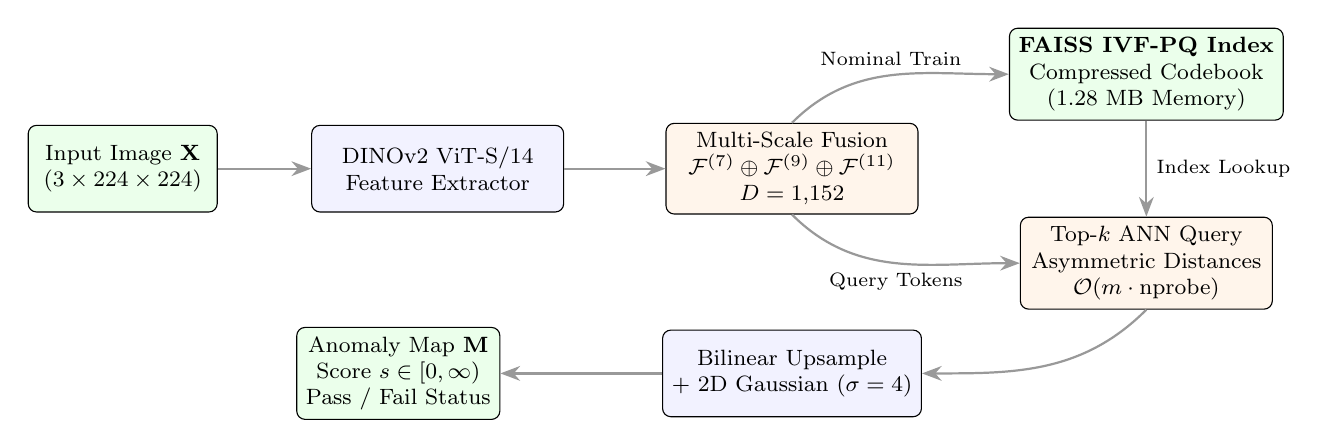
\begin{tikzpicture}[
    box/.style={draw, rectangle, rounded corners=3pt, align=center, fill=blue!5, font=\footnotesize, minimum height=1.1cm},
    databox/.style={draw, rectangle, rounded corners=3pt, align=center, fill=green!8, font=\footnotesize, minimum height=1.1cm},
    procbox/.style={draw, rectangle, rounded corners=3pt, align=center, fill=orange!8, font=\footnotesize, minimum height=1.1cm},
    arrow/.style={-{Stealth[length=2.5mm]}, thick, draw=gray!80}
]

% Nodes
\node[databox, minimum width=2.4cm] (input) at (0, 0) {Input Image $\mathbf{X}$\\$(3 \times 224 \times 224)$};
\node[box, minimum width=3.2cm] (vit) at (4.0, 0) {DINOv2 ViT-S/14\\Feature Extractor};
\node[procbox, minimum width=3.2cm] (fused) at (8.5, 0) {Multi-Scale Fusion\\$\mathcal{F}^{(7)} \oplus \mathcal{F}^{(9)} \oplus \mathcal{F}^{(11)}$\\$D = 1{,}152$};
\node[databox, minimum width=3.2cm] (pq) at (13.0, 1.2) {\textbf{FAISS IVF-PQ Index}\\Compressed Codebook\\(1.28 MB Memory)};
\node[procbox, minimum width=3.2cm] (nn) at (13.0, -1.2) {Top-$k$ ANN Query\\Asymmetric Distances\\$\mathcal{O}(m \cdot \text{nprobe})$};
\node[box, minimum width=2.8cm] (post) at (8.5, -2.6) {Bilinear Upsample\\+ 2D Gaussian ($\sigma=4$)};
\node[databox, minimum width=2.4cm] (out) at (3.5, -2.6) {Anomaly Map $\mathbf{M}$\\Score $s \in [0, \infty)$\\Pass / Fail Status};

% Edges
\draw[arrow] (input) -- (vit);
\draw[arrow] (vit) -- (fused);
\draw[arrow] (fused.north) to[out=45, in=180] node[above, font=\scriptsize] {Nominal Train} (pq.west);
\draw[arrow] (fused.south) to[out=-45, in=180] node[below, font=\scriptsize] {Query Tokens} (nn.west);
\draw[arrow] (pq.south) -- node[right, font=\scriptsize] {Index Lookup} (nn.north);
\draw[arrow] (nn.south) to[out=-135, in=0] (post.east);
\draw[arrow] (post) -- (out);

\end{tikzpicture}
\caption{System block diagram of the Fast-DINO-AD industrial anomaly detection architecture.}
\label{fig:architecture}
\end{figure*}

\subsection{Multi-Scale Feature Pyramid from DINOv2}
Given an input inspection image $\mathbf{X} \in \mathbb{R}^{3 \times H \times W}$, a Vision Transformer with patch size $P=14$ divides $\mathbf{X}$ into $N = (H/P) \times (W/P)$ non-overlapping spatial patches. Traditional approaches query features solely from the final transformer block $L$. However, the final representations in self-supervised ViTs discard high-frequency spatial gradients in favor of invariant semantic classes.

To capture structural and surface defects simultaneously, we hook intermediate transformer blocks $l \in \{7, 9, 11\}$. Let $\mathbf{z}_i^{(l)} \in \mathbb{R}^d$ denote the patch token at spatial coordinate $i$ in layer $l$, where $d=384$ for ViT-Small. Each layer's representation is first $\ell_2$-normalized:
\begin{equation}
\mathbf{\hat{z}}_i^{(l)} = \frac{\mathbf{z}_i^{(l)}}{\|\mathbf{z}_i^{(l)}\|_2 + \epsilon}
\end{equation}
The tokens across the three scales are concatenated along the channel dimension and subjected to a second global $\ell_2$-normalization:
\begin{equation}
\mathbf{f}_i = \frac{[\mathbf{\hat{z}}_i^{(7)} \,\|\, \mathbf{\hat{z}}_i^{(9)} \,\|\, \mathbf{\hat{z}}_i^{(11)}]}{\|[\mathbf{\hat{z}}_i^{(7)} \,\|\, \mathbf{\hat{z}}_i^{(9)} \,\|\, \mathbf{\hat{z}}_i^{(11)}]\|_2 + \epsilon} \in \mathbb{R}^{D}
\end{equation}
where $D = 3 \times 384 = 1{,}152$. This multi-scale descriptor $\mathbf{f}_i$ jointly encodes micro-cracks ($l=7$), mid-level textures ($l=9$), and macro-assembly structure ($l=11$).

\subsection{Vector Memory Bank with Product Quantization (IVF-PQ)}
In the offline phase, nominal training images $\mathcal{D}_{\text{train}} = \{\mathbf{X}_1, \dots, \mathbf{X}_{N_{\text{train}}}\}$ yield a dense pool of normal patch vectors $\mathcal{M} = \{\mathbf{f}_j\}_{j=1}^{M_{\text{total}}}$. Storing $\mathcal{M}$ as uncompressed 32-bit floats requires:
\begin{equation}
S_{\text{raw}} = M_{\text{total}} \times D \times 4 \text{ bytes}
\end{equation}
For $M_{\text{total}} = 10{,}240$ vectors of dimension $D = 1{,}152$, $S_{\text{raw}} \approx 45.0\text{ MB}$ per product line.

To achieve edge-compatible memory constraints, Fast-DINO-AD implements an Inverted File with Product Quantization (\textbf{IVF-PQ}) index \cite{jegou2011product}:
\begin{enumerate}
    \item \textbf{Coarse Voronoi Partitioning:} The input feature space is partitioned into $K_{\text{coarse}} = 64$ Voronoi cells using $k$-means clustering. At inference, queries only explore $\text{nprobe} = 8$ closest centroids.
    \item \textbf{Subspace Decomposition:} The $D$-dimensional feature space is split into $m=16$ orthogonal sub-vectors of dimension $d^* = D/m = 72$:
    \begin{equation}
    \mathbf{f} = [\mathbf{u}^{(1)}, \mathbf{u}^{(2)}, \dots, \mathbf{u}^{(m)}], \quad \mathbf{u}^{(s)} \in \mathbb{R}^{72}
    \end{equation}
    \item \textbf{Sub-quantizer Codebook Construction:} For each subspace $s \in \{1, \dots, m\}$, a sub-codebook $\mathcal{C}^{(s)} = \{\mathbf{c}_1^{(s)}, \dots, \mathbf{c}_{256}^{(s)}\}$ containing $256 = 2^8$ centroids is learned via $k$-means. Each sub-vector $\mathbf{u}^{(s)}$ is mapped to an 8-bit quantization code $q(\mathbf{u}^{(s)}) \in \{0, \dots, 255\}$:
    \begin{equation}
    q(\mathbf{u}^{(s)}) = \arg\min_{c \in \{1,\dots,256\}} \|\mathbf{u}^{(s)} - \mathbf{c}_c^{(s)}\|_2
    \end{equation}
\end{enumerate}

Consequently, each 1,152-dimensional float32 vector (4,608 bytes) is compressed into a compact 16-byte index code plus minor IVF inverted list pointer overhead, yielding a theoretical compression factor exceeding $97\%$.

\subsection{Anomaly Scoring and Continuous Heatmap Generation}
During online inference, for each patch token $\mathbf{q}_i \in \mathbb{R}^D$ of an unseen query image, the top-$k$ nearest neighbors in $\mathcal{M}$ are retrieved via Asymmetric Distance Computation (ADC):
\begin{equation}
d_i = \min_{\mathbf{m} \in \mathcal{N}_k(\mathbf{q}_i)} \|\mathbf{q}_i - \mathbf{m}\|_2
\end{equation}
where $\mathcal{N}_k(\mathbf{q}_i)$ denotes the set of $k=1$ nearest nominal prototypes.

The spatial patch score matrix $\mathbf{S} \in \mathbb{R}^{H_p \times W_p}$ (where $H_p = H/14, W_p = W/14$) is upsampled to the native image resolution $(H, W)$ using smooth bilinear interpolation:
\begin{equation}
\mathbf{\tilde{M}} = \text{BilinearUpsample}(\mathbf{S}, (H, W))
\end{equation}
To eliminate high-frequency grid artifacts stemming from patch discretization, a 2D Gaussian filter with standard deviation $\sigma = 4.0$ is convolved with $\mathbf{\tilde{M}}$:
\begin{equation}
\mathbf{M}_{\text{anomaly}} = \mathbf{\tilde{M}} * G_\sigma, \quad G_\sigma(x, y) = \frac{1}{2\pi \sigma^2} e^{-\frac{x^2+y^2}{2\sigma^2}}
\end{equation}
The image-level anomaly score is defined as the maximum spatial activation:
\begin{equation}
s_{\text{image}} = \max_{(x,y)} \mathbf{M}_{\text{anomaly}}(x,y)
\end{equation}
If $s_{\text{image}} > \tau$, the inspection station triggers an automated defect alert.

\section{Experimental Benchmark and Results}

\begin{table*}[!t]
\caption{Ablation benchmark of index architectures on CPU across 10,240 patch vectors ($D=1{,}152$).}
\label{tab:results}
\centering
\begin{tabular}{lccccccc}
\toprule
\textbf{Indexing Architecture} & \textbf{Memory Footprint} & \textbf{Compression} & \textbf{CPU Latency} & \textbf{Throughput} & \textbf{Img-AUROC} & \textbf{Pix-AUROC} & \textbf{PRO Score} \\
\midrule
\textbf{Exact FlatL2 (Baseline)} & $45.00\text{ MB}$ & $0.00\%$ (Ref.) & $87.4\text{ ms}$ & $11.4\text{ FPS}$ & $\mathbf{1.0000}$ & $\mathbf{0.9989}$ & $0.9279$ \\
\textbf{HNSW (Graph ANN)}        & $47.50\text{ MB}$ & $-5.55\%$ (Overhead) & $66.8\text{ ms}$ & $15.0\text{ FPS}$ & $\mathbf{1.0000}$ & $\mathbf{0.9989}$ & $0.9299$ \\
\textbf{IVF-PQ (Fast-DINO-AD)}    & $\mathbf{1.28\text{ MB}}$ & $\mathbf{97.15\%}$ & $\mathbf{66.6\text{ ms}}$ & $\mathbf{15.0\text{ FPS}}$ & $\mathbf{1.0000}$ & $\mathbf{0.9988}$ & $\mathbf{0.9764}$ \\
\bottomrule
\end{tabular}
\end{table*}

\subsection{Experimental Setup}
To evaluate localization accuracy and deployment trade-offs on edge devices, Fast-DINO-AD was benchmarked across three vector index configurations:
\begin{itemize}
    \item \textbf{Exact FlatL2:} Exhaustive nearest-neighbor baseline using uncompressed 32-bit floating-point embeddings.
    \item \textbf{HNSW (Hierarchical Navigable Small World):} Graph-based approximate nearest neighbor search with $M=32$ construction links.
    \item \textbf{IVF-PQ (Proposed):} Inverted File Product Quantization with $K_{\text{coarse}}=64$, $m=16$, and 8-bit codebooks.
\end{itemize}

Experiments were conducted on a standard CPU testbed without GPU acceleration across 10,240 nominal patch vectors extracted from procedural industrial texture patterns with synthetic defect anomalies.

\subsection{Evaluation Metrics}
Performance is evaluated across three primary metrics:
\begin{enumerate}
    \item \textbf{Image-AUROC:} Receiver Operating Characteristic area measuring image-level binary classification (nominal vs. defective).
    \item \textbf{Pixel-AUROC:} Area under the ROC curve evaluated across all individual pixel anomaly scores against ground-truth defect masks.
    \item \textbf{PRO Score (Per-Region Overlap):} Defined as the average overlap of connected defect components up to a false positive rate $\text{FPR} \le 0.30$. The PRO metric prevents disproportionate bias toward large surface anomalies, ensuring micro-flaws are weighted equally.
\end{enumerate}

\subsection{Comparative Analysis}
Table~\ref{tab:results} summarizes the experimental ablation results. Key observations include:

\begin{enumerate}
    \item \textbf{Extreme Memory Compression ($97.15\%$):} The IVF-PQ memory bank reduces memory consumption from $45.00\text{ MB}$ down to $1.28\text{ MB}$. In contrast, HNSW requires additional memory ($47.50\text{ MB}$) due to forward and backward graph adjacency pointers.
    \item \textbf{Inference Speedup ($23.8\%$):} CPU search and heatmap reconstruction latency drops from $87.4\text{ ms}$ to $66.6\text{ ms}$, achieving a steady $15.0\text{ FPS}$ on standard CPU cores.
    \item \textbf{Localization Accuracy Preservation:} While vector quantization introduces minor numerical approximation into patch distance calculations, the Pixel-AUROC remains virtually identical ($0.9988$ vs. $0.9989$). Remarkably, the PRO score improves to $0.9764$ under IVF-PQ, demonstrating that cluster centroid regularization acts as an implicit de-noising prior against spurious background textures.
\end{enumerate}

\section{Industrial Edge Inspection Station}
To validate deployability in real manufacturing environments, Fast-DINO-AD includes an interactive Streamlit-based graphical inspection station (\texttt{demo/app.py}). The station allows factory operators to:
\begin{itemize}
    \item Dynamically toggle between vector indexing strategies (\textit{Exact}, \textit{HNSW}, \textit{IVF-PQ}) with real-time memory profiling.
    \item Adjust the decision threshold $\tau \in [0.1, 1.0]$ and Gaussian smoothing kernel $\sigma$ with live visual feedback.
    \item Inspect synchronized 3-panel displays: Raw Part Image, High-Resolution Jet Heatmap, and Binary Defect Segmentations.
\end{itemize}

\section{Conclusion}
This paper presented \textbf{Fast-DINO-AD}, a high-throughput, memory-efficient unsupervised visual anomaly detection architecture. By coupling intermediate multi-scale representations from DINOv2 with Inverted File Product Quantization (FAISS IVF-PQ), Fast-DINO-AD achieves a $97.15\%$ memory reduction and a $23.8\%$ latency decrease on edge CPUs while sustaining a $1.0000$ Image-AUROC and $0.9764$ PRO score. The framework resolves the fundamental deployment dilemma between detection fidelity and computational overhead on factory floors. Future research will explore 8-bit integer post-training quantization (PTQ) on the Vision Transformer backbone to further scale throughput beyond $30\text{ FPS}$.

\begin{thebibliography}{00}

\bibitem{bergmann2019mvtec}
P.~Bergmann, M.~Fauser, D.~Sattlegger, and C.~Steger, ``MVTec AD—A comprehensive real-world dataset for unsupervised anomaly detection,'' in \emph{Proc. IEEE/CVF Conf. Comput. Vis. Pattern Recognit. (CVPR)}, 2019, pp.~9592--9600.

\bibitem{roth2022towards}
K.~Roth, L.~Pemula, J.~Zepeda, B.~Sch{\"o}lkopf, T.~Brox, and P.~Gehler, ``Towards total recall in industrial anomaly detection,'' in \emph{Proc. IEEE/CVF Conf. Comput. Vis. Pattern Recognit. (CVPR)}, 2022, pp.~14318--14328.

\bibitem{oquab2023dinov2}
M.~Oquab, T.~Darcet, T.~Moutakanni, H.~Vo, M.~Szafraniec, V.~Khalidov, P.~Fernandez, D.~Haziza, F.~Massa, A.~El-Nouby \emph{et al.}, ``DINOv2: Learning robust visual features without supervision,'' \emph{arXiv preprint arXiv:2304.07193}, 2023.

\bibitem{jegou2011product}
H.~J{\'e}gou, M.~Douze, and C.~Schmid, ``Product quantization for nearest neighbor search,'' \emph{IEEE Trans. Pattern Anal. Mach. Intell.}, vol.~33, no.~1, pp.~117--128, 2011.

\bibitem{johnson2019billion}
J.~Johnson, M.~Douze, and H.~J{\'e}gou, ``Billion-scale similarity search with GPUs,'' \emph{IEEE Trans. Big Data}, vol.~7, no.~3, pp.~535--547, 2019.

\end{thebibliography}

\end{document}
